\documentclass[11pt,a4paper]{article}

\usepackage[spanish,es-tabla]{babel}
\usepackage[utf8]{inputenc}
\usepackage[T1]{fontenc}
\usepackage{lmodern}
\usepackage{microtype}
\usepackage{graphicx}
\usepackage{booktabs}
\usepackage{tabularx}
\usepackage{array}
\usepackage{siunitx}
\usepackage{xcolor}
\usepackage[hidelinks]{hyperref}
\usepackage[margin=2.6cm]{geometry}
\usepackage[font=small,labelfont=bf]{caption}
\usepackage{subcaption}
\usepackage{enumitem}
\usepackage{csquotes}

\sisetup{detect-all=true}
\graphicspath{{figures/}}
\setlist[itemize]{leftmargin=*, itemsep=0.2em}
\setlist[enumerate]{leftmargin=*, itemsep=0.2em}

\newcommand{\run}[1]{\nolinkurl{#1}}
\newcommand{\metric}[1]{\nolinkurl{#1}}

\title{\textbf{Foraging multi-agente con memoria externa en grillas: un estudio experimental}}
\author{Jeremías Figueiredo Paschmann \and Francisco Nattero \and Juan Kaplan}
\date{Proyecto final de Aprendizaje por Refuerzo}

\begin{document}
\maketitle

\begin{abstract}
Este informe reconstruye una serie de experimentos de aprendizaje por refuerzo multi-agente en un entorno de foraging con memoria externa discreta. La tarea exige que agentes con observación local encuentren fuentes de comida, transporten unidades al hub y sostengan ciclos de entrega bajo ejecución descentralizada. La evidencia muestra que el progreso no se explica por aumentar la cantidad de bits de comunicación, sino por una secuencia de cambios más concreta: corregir el contrato de la tarea, hacer aprendible la señal de crédito, aumentar la cobertura con más agentes y reemplazar el crítico centralizado plano por una arquitectura espacial. En 25x25 se obtuvo una política que completa las 23 entregas bajo movimiento muestreado. En 50x50, la frontera más fuerte aparece dentro de la familia con crítico \run{strided_cnn}, donde una política de 60 hormigas alcanza una fracción de entrega cercana a 0.99 en evaluación seleccionada, aunque esa mejora queda confundida con cantidad de agentes, identidades, selección de checkpoints y escritura casi saturada. En 250x250, el resultado más importante es negativo: el retorno moldeado y la actividad de bytes pueden crecer aunque las entregas reales sigan siendo nulas. Para evitar una historia retrospectiva demasiado limpia, se auditó el checkout completo y se clasificaron commits, refs, notebooks, configuraciones, corridas locales, carpetas W\&B, logs y artefactos por familia experimental. La conclusión es deliberadamente acotada: el sistema aprendió foraging cooperativo útil y escaló a escenarios 50x50 exigentes, pero todavía no demuestra causalmente comunicación emergente mediante la memoria por bytes.
\end{abstract}

\begin{figure}[h]
\centering
\fbox{\begin{minipage}{0.94\linewidth}
\small
\centering
\begin{tabularx}{\linewidth}{>{\centering\arraybackslash}X c >{\centering\arraybackslash}X c >{\centering\arraybackslash}X c >{\centering\arraybackslash}X}
\textbf{Contrato} & \(\Longrightarrow\) & \textbf{Crédito} & \(\Longrightarrow\) & \textbf{Crítico} & \(\Longrightarrow\) & \textbf{Conclusión} \\
entregas reales con fuentes agotables
&
&
moldeado de distancia, más agentes y evaluación muestreada
&
&
crítico espacial, checkpoints seleccionados y auditoría por familia
&
&
foraging fuerte sin prueba causal de comunicación por bytes
\end{tabularx}
\end{minipage}}
\caption{Resumen gráfico del argumento central. La lectura del proyecto va desde la definición correcta de la tarea hasta la interpretación causal de los resultados: las métricas de entrega explican el desempeño, la arquitectura del crítico explica parte del salto 50x50 y las ablaciones de memoria delimitan lo que todavía no puede afirmarse.}
\label{fig:graphical-abstract}
\end{figure}

\section{Introducción}

El problema que se estudia es simple de describir y difícil de aprender: varios agentes locales deben encontrar fuentes de comida, recoger unidades de comida y volver al hub para entregarlas. Cada agente observa solo una vecindad pequeña y ejecuta una política compartida. Durante el entrenamiento se permite un crítico centralizado, pero durante el despliegue la política sigue siendo local. Esta separación corresponde al marco de entrenamiento centralizado con ejecución descentralizada, usado en algoritmos multi-agente como MAPPO y MADDPG \cite{yu2022mappo,lowe2017maddpg}.

La motivación no es solo maximizar una métrica. La pregunta relevante es semántica: qué comportamiento aparece cuando se combinan búsqueda local, memoria en el ambiente y presión de entregar comida. Un resultado útil no debería ser únicamente ``alto reward'', sino que debería mostrar ciclos completos de foraging, retorno al hub, uso razonable del espacio y robustez bajo mapas aleatorios. Por eso el análisis separa tres capas que suelen mezclarse. La primera es el desempeño, medido por comida entregada, tasa de éxito y eficiencia temporal. La segunda es el mecanismo, es decir, los cambios de entorno, política, crítico o evaluación que hicieron posible ese desempeño. La tercera es el comportamiento visible: si los videos muestran búsqueda, transporte y retorno, o si solo muestran movimiento local sostenido por retorno moldeado.

El trabajo se ubica cerca de MAPPO \cite{yu2022mappo}, PPO \cite{schulman2017ppo}, GAE \cite{schulman2015gae} y aprendizaje de comunicación multi-agente como CommNet y DIAL \cite{sukhbaatar2016commnet,foerster2016dial}. La diferencia práctica es que aquí la comunicación no es un canal diferentiable directo entre agentes. Es una memoria discreta escrita en celdas del ambiente. Eso hace que la atribución causal sea más difícil: ver bytes no-cero no implica que esos bytes estén coordinando la política.

\section{Entorno experimental}

La semántica del entorno cambió de manera decisiva durante el proyecto. En la versión relevante para este informe, \metric{food_count} no significa posiciones independientes de comida. Significa mordidas totales. \metric{food_sources} controla cuántas fuentes concentran esas mordidas y cada fuente se agota. La recompensa cruda principal es la entrega en el hub: una unidad entregada da \(+1\). La recogida puede tener bonus de moldeado en algunas corridas, pero no es el objetivo final.

Esta distinción cambia la interpretación de todos los resultados. Un resultado de \(23/23\) en 25x25 no significa visitar 23 puntos aislados. Significa completar 23 entregas desde 6 fuentes agotables. Cambiar \metric{food_sources} con \metric{food_count} fijo cambia la geometría de la tarea, la repetición de rutas y la dificultad de redescubrir fuentes.

\begin{table}[h]
\centering
\caption{Variables semánticas que no deben tratarse como detalles menores.}
\begin{tabularx}{\linewidth}{>{\raggedright\arraybackslash}p{0.28\linewidth}X}
\toprule
Variable & Interpretación para el informe \\
\midrule
\metric{food_count} & Total de unidades que pueden ser entregadas. Es el denominador natural de la fracción entregada. \\
\metric{food_sources} & Número de fuentes agotables. A igual \metric{food_count}, menos fuentes implican fuentes más densas. \\
\metric{sampled movement} & Despliegue estocástico de movimiento. Muchas políticas buenas viven en la distribución, no en el argmax. \\
\metric{greedy movement} & Despliegue determinista. Es más estricto y frecuentemente empeora el retorno. \\
\metric{critic_architecture} & Arquitectura del crítico centralizado. Cambia la señal de valor durante PPO aunque el actor local no reciba observación global en ejecución. \\
\metric{write_while_moving} & Permite escribir mientras se mueve. Cambia el costo y la frecuencia efectiva de escritura. \\
\bottomrule
\end{tabularx}
\end{table}

\section{Método}

La base de entrenamiento es PPO multi-agente con política compartida, ventajas estimadas con GAE y un crítico centralizado. PPO optimiza una función objetivo recortada que evita cambios demasiado grandes de política \cite{schulman2017ppo}. MAPPO aplica esta idea a agentes cooperativos y suele usar un crítico centralizado para estabilizar el aprendizaje \cite{yu2022mappo}. En este proyecto, el actor debe ejecutar con información local; el crítico puede ver más información durante entrenamiento.

La arquitectura del crítico es una frontera causal del proyecto. Las líneas tempranas y el 50x50 eficiente inicial usaron un crítico \run{mlp} plano sobre observaciones centralizadas aplanadas. La línea posterior de proximidad y full-layout en 50x50 introdujo \run{strided_cnn}, un crítico espacial que procesa planos de grilla y rasgos de entidades. Los diagnósticos 250x250 pertenecen a una familia distinta, donde aparecen críticos \run{resnet_cnn}, \run{strided_cnn} y \run{set_cnn} bajo contratos de escala y reset diferentes. Esta separación impide presentar los resultados como si todos fueran puntos de una única curva de comunicación.

Esta separación es central. Si una corrida 50x50 mejora después de pasar de \run{mlp} a \run{strided_cnn}, no se puede atribuir la mejora solamente a más hormigas, más bits, fuentes más densas o escritura compartida. El crítico cambió el problema de crédito que PPO resuelve durante entrenamiento.

Cada corrida se leyó como un conjunto de artefactos, no como una captura aislada. El contrato de tarea queda en \run{experiments/*.json} o en el notebook que arma la corrida. La traza temporal queda en \run{metrics.jsonl}. El cierre queda en \run{summary.json}. Los pesos quedan en checkpoints finales y, cuando se activó selección, en checkpoints ``best''. Los videos de W\&B o locales sirven como evidencia cualitativa sincronizada con updates o checkpoints, pero no reemplazan las métricas de tarea.

Esta trazabilidad importa porque ``best checkpoint'' no significa ``último checkpoint''. El runner puede seleccionar por una métrica de entrenamiento o de evaluación, en modo máximo o mínimo, y las evaluaciones pueden usar semillas desplazadas, layouts barajados y modos de acción como movimiento muestreado con escritura greedy. Por eso el informe separa cuatro niveles: configuración, curva de entrenamiento, evaluación seleccionada y video. El sitio web que acompaña al informe agrega una quinta capa de inspección: un visor de artefactos y un simulador interactivo del actor 50x50 exportado a JavaScript. Ese simulador permite cambiar tamaño de grilla, cantidad de hormigas, unidades de comida, posiciones de fuente y paleta visual, pero sigue siendo ejecución solo-actor: sin crítico, sin JAX y sin entrenamiento. Sirve para inspeccionar una política local ya entrenada, no para crear una nueva corrida comparable.

La misma regla se aplica a los videos nuevos del sitio. Cada video debe indicar de qué checkpoint viene, qué modo de acción usa y si el entorno cambia el contrato original. En mapas con paredes, las paredes se pasan al actor por el canal local de borde/obstáculo, implementado como \run{local_border = max(border, obstacles)}. Por lo tanto, un fracaso en laberinto no significa automáticamente que el actor no observe paredes; puede significar que una política entrenada en foraging abierto no aprendió el comportamiento necesario para navegar pasillos internos.

\begin{table}[h]
\centering
\caption{Cómo se interpreta una corrida en este informe.}
\begin{tabularx}{\linewidth}{>{\raggedright\arraybackslash}p{0.22\linewidth}X>{\raggedright\arraybackslash}p{0.26\linewidth}}
\toprule
Artefacto & Qué fija & Riesgo si se omite \\
\midrule
\run{config.json} o \run{experiments/*.json} & Tamaño, fuentes, comida, hormigas, bits, radio, crítico, horizonte, rewards y modo de transferencia. & Comparar corridas que no tienen el mismo contrato. \\
\run{metrics.jsonl} & Evolución por update: entregas, pickups, cobertura, bytes, entropía, KL, gradientes y pérdidas. & Confundir un pico, una caída o una métrica moldeada con desempeño final. \\
\run{summary.json} & Estado final y, cuando existe, métricas del mejor checkpoint. & Mezclar último checkpoint con checkpoint seleccionado. \\
Videos locales / W\&B & Comportamiento visible: búsqueda, recogida, regreso al hub, saturación de bytes o movimiento sin entrega. & Usar un video vistoso como sustituto de eventos reales. \\
\bottomrule
\end{tabularx}
\end{table}

\subsection{Auditoría de árbol y ramas visibles}

Para que el informe y el sitio no cuenten solo los resultados más presentables, se generó un ledger exhaustivo en \run{docs/planning/experiment-tree-audit}. La auditoría tomó como base el checkout limpio en \run{21d3cdf} y clasificó cada commit alcanzable, cada ref visible, cada configuración actual, cada notebook, cada directorio local de evidencia, cada run W\&B local y cada archivo experimental indexable. La salida no reemplaza la interpretación causal; fija el inventario de lo que existe y obliga a ubicar incluso las ramas que no dejaron un resultado final comparable.

\begin{table}[h]
\centering
\caption{Cobertura del ledger de auditoría usado para actualizar el árbol.}
\begin{tabularx}{\linewidth}{>{\raggedright\arraybackslash}p{0.26\linewidth}>{\raggedright\arraybackslash}p{0.18\linewidth}X}
\toprule
Superficie auditada & Cantidad & Qué significa para la lectura \\
\midrule
Commits alcanzables & 334 & Historia completa visible desde refs locales y remotos. \\
Refs visibles & 13 & Incluye ramas fusionadas, rama del sitio e investigaciones no fusionadas. \\
Cambios path-level & 1651 & Permite ubicar cada cambio de archivo dentro de una familia experimental. \\
Configs \run{experiments/*.json} & 25 & Contratos explícitos de entrenamiento y evaluación. \\
Notebooks & 17 & Superficies de lanzamiento, análisis, videos y exploración. \\
Directorios de runs & 145 & Evidencia local con summaries, métricas, evals, planes o configs. \\
Runs W\&B locales & 230 & Carpetas locales indexadas; el API cloud quedó bloqueado por \run{relogin required}. \\
Logs & 9 & Registros operacionales preservados. \\
Archivos indexados & 7771 & Superficie del checkout fuera de \run{.git}, entornos locales y la propia salida de auditoría. \\
\bottomrule
\end{tabularx}
\end{table}

\begin{table}[p]
\centering
\scriptsize
\caption{Familias del árbol completo. La columna ``ubicación'' indica cómo deben aparecer en el sitio y en la lectura del informe, no una afirmación causal.}
\begin{tabularx}{\linewidth}{>{\raggedright\arraybackslash}p{0.38\linewidth}>{\raggedright\arraybackslash}p{0.16\linewidth}X}
\toprule
Familia & Evidencia & Ubicación en el árbol \\
\midrule
\run{foundation-task-contract} & 8 commits, 11 archivos & Nacimiento del entorno: sprites, reset, fuentes agotables, entrega y rollout aleatorio. \\
\run{jax-mappo-training-core} & 21 commits, 155 archivos, 13 W\&B locales & JAX, MAPPO, trainer, eval, checkpoints, recursos y ramas multi-device. \\
\run{autocurriculum-exploration-baselines} & 29 commits, 4 configs, 4 notebooks & Forage/exploration/autocurrículos tempranos y lanzadores base. \\
\run{communication-memory-bytes} & 94 commits, 10 runs, 27 W\&B locales & Bits, memoria externa, write-head, no-write, write-cost y R8--R12. \\
\run{ant-count-25x25-autoresearch} & 75 commits, 52 runs & Desbloqueo 25x25 por distancia, cobertura, cantidad de hormigas, CAP y visión. \\
\run{source-layout-50x50} & 4 commits, 4 configs, 4 notebooks & Fuente sparse 50x50: padded, proximity, smooth, rare, vectores y previews. \\
\run{critic-full-layout-50x50} & 29 commits, 6 configs, 3 runs & Cambio a crítico espacial, full-layout, shared writes, costo y continuaciones 8-ant. \\
\run{sixty-ant-50x50-stabilization} & 6 commits, 4 configs, 1 notebook & Frontera 50x50 con 60 hormigas, 8 bits, identidad y estabilización. \\
\run{hundred-bridge-maze-stress} & 16 commits, 16 runs, 173 W\&B locales & Puente 100x100, laberinto entrenado como exploración y stress maze 100x100. \\
\run{twofifty-frontier-reset} & 15 commits, 25 runs, 11 W\&B locales & 250x250, half-scale, resnet/set critics, reset-boundary, truncación y distancia. \\
\run{bigmap-deployment-rendering} & 10 commits, 6 runs & Render y despliegue solo-actor grande: 1000x1000, paletas y sandbox JS. \\
\run{adversarial-roles-side-branches} & 14 commits & Frozen-opponent, timed-release roles y probes visibles solo por branch. \\
\run{report-site-paper-assets} & 8 commits, 65 archivos & Informe, sitio, plots, videos, posters, planificación y figuras generadas. \\
\run{infra-tests-ci-cleanup} & 3 commits, 522 archivos, 31 runs & Tests, CI, packaging, limpieza de almacenamiento y soporte no experimental. \\
\run{curated-results-and-vault} & 4 archivos & Índices curados y placeholders de vault; evidencia retenida, no experimento nuevo. \\
\run{unclassified-review-needed} & 2 commits & Bucket explícito para evidencia que no debe usarse en el paper sin inspección manual. \\
\bottomrule
\end{tabularx}
\end{table}

\begin{table}[p]
\centering
\scriptsize
\caption{Refs visibles que fijan ramas del árbol. Las ramas no fusionadas se documentan como evidencia o dirección exploratoria, no como resultados comparables salvo que tengan métricas preservadas.}
\begin{tabularx}{\linewidth}{>{\raggedright\arraybackslash}p{0.34\linewidth}>{\raggedright\arraybackslash}p{0.35\linewidth}X}
\toprule
Ref & Familia & Lectura \\
\midrule
\run{main}, \run{origin/main}, \run{origin/HEAD} & \run{critic-full-layout-50x50} & Base remota fusionada con la línea de crítico/full-layout 50x50. \\
\run{report-writing-site}, \run{origin/report-writing-site} & \run{report-site-paper-assets} & Rama actual del informe, sitio, videos, plots y árbol narrativo. \\
\run{feat/multi-device-jax-mappo}, \run{origin/feat/multi-device-jax-mappo} & \run{jax-mappo-training-core} & Rendimiento/multi-device y experimentos x150/write-cost; no se lee como resultado principal. \\
\run{train-half-scale-resnet} & \run{twofifty-frontier-reset} & Lanzamiento half-scale resnet 250x250: dirección de escala, no resultado final comparable. \\
\run{origin/lethal_cookies} & \run{hundred-bridge-maze-stress} & Arena en L, laberinto/proximidad y bolsillos letales; sin métricas locales finales comparables. \\
\run{origin/research/adversarial-marl-experiments} & \run{adversarial-roles-side-branches} & Frozen-opponent y roles adversariales documentados como probes laterales. \\
\run{origin/research/timed-release-roles} & \run{adversarial-roles-side-branches} & Continuación parked de roles cooperativos con liberación temporal. \\
\run{origin/vision_shrink_curriculum} & \run{ant-count-25x25-autoresearch} & Continuación CAP/visión de 25x25; pertenece al árbol de cobertura, no a la frontera 50x50. \\
\run{origin/repo/research-integration-cleanup} & \run{jax-mappo-training-core} & Integración, tests y limpieza de soporte; relevante para reproducibilidad. \\
\bottomrule
\end{tabularx}
\end{table}

Las figuras siguen un criterio editorial simple: el lienzo del gráfico se reserva para datos, ejes, leyendas, umbrales y anotaciones numéricas. La interpretación de cada resultado aparece en la leyenda y en el texto que acompaña a la figura, no como un título incrustado dentro del gráfico.

\section{Resultados experimentales}

\subsection{Cambio de contrato de la tarea}

El primer cambio grande fue conceptual. La tarea dejó de premiar fuertemente recoger comida y pasó a medir entregas al hub con fuentes agotables. Esto convirtió el problema en foraging real: encontrar no basta, hay que cerrar el ciclo fuente-hub. También hizo que la densidad de fuentes fuera una variable de dificultad.

Esta frontera invalida comparaciones ingenuas con corridas viejas. Un reward alto bajo pickup reward no significa lo mismo que un reward alto bajo delivery-only reward.

\subsection{Primer enfoque: mapas cada vez más grandes}

La primera línea JAX intentó resolver el problema como un currículo de tamaño: entrenar en mapas chicos y aumentar progresivamente hasta 50x50. El contrato de \run{forage_curriculum.json} era una hormiga, radio local 1, 48 unidades de comida repartidas en 12 fuentes, 1 bit de escritura, 10000 pasos máximos, \run{hidden_size}=128 y etapas explícitas de 4x4 a 50x50. Era una idea razonable: si la política aprende el ciclo fuente-hub en chico, tal vez pueda transferirlo a mapas más grandes.

No alcanzó. El reporte consolidado local registra que el retorno bajaba de \(12.281\) en 4x4 a \(0.719\) en 25x25 y \(0.156\) en 50x50. El patrón observado era compatible con agentes que exploran o cargan comida, pero no convierten eso en ciclos repetidos de entrega.

También quedó preservada una secuencia posterior de checkpoints de tamaño, de 8x8 a 50x50, con 4 hormigas, 1 bit, radio 1 y observación 50x50. Esa secuencia visual es útil porque muestra el contrato experimental creciendo, no porque resuelva la frontera. En esa corrida, el mejor punto evaluado llegó a \(22.5/48\) y \(0.9\) entregas por 1000 pasos-hormiga, pero la familia volvió a oscilar y no quedó como solución robusta. La causa más plausible no fue falta de bits. Era una mezcla de horizonte largo, recompensa escasa, cobertura insuficiente y crédito débil.

\subsection{El desbloqueo 25x25}

El primer resultado fuerte aparece al combinar moldeado de distancia, más hormigas y más capacidad. \run{DISTANCE_SHAPE} ya hacía parcialmente aprendible el umbral 25x25: \(13.75/23\) en greedy, pero solo \(7/23\) muestreado. \run{DISTANCE_CAP4} cambia a cuatro hormigas y hidden size mayor; allí la evaluación muestreada llega a \(23/23\) con éxito \(1.0\), aunque el modo greedy cae a \(2.75/23\).

\begin{figure}[h]
\centering
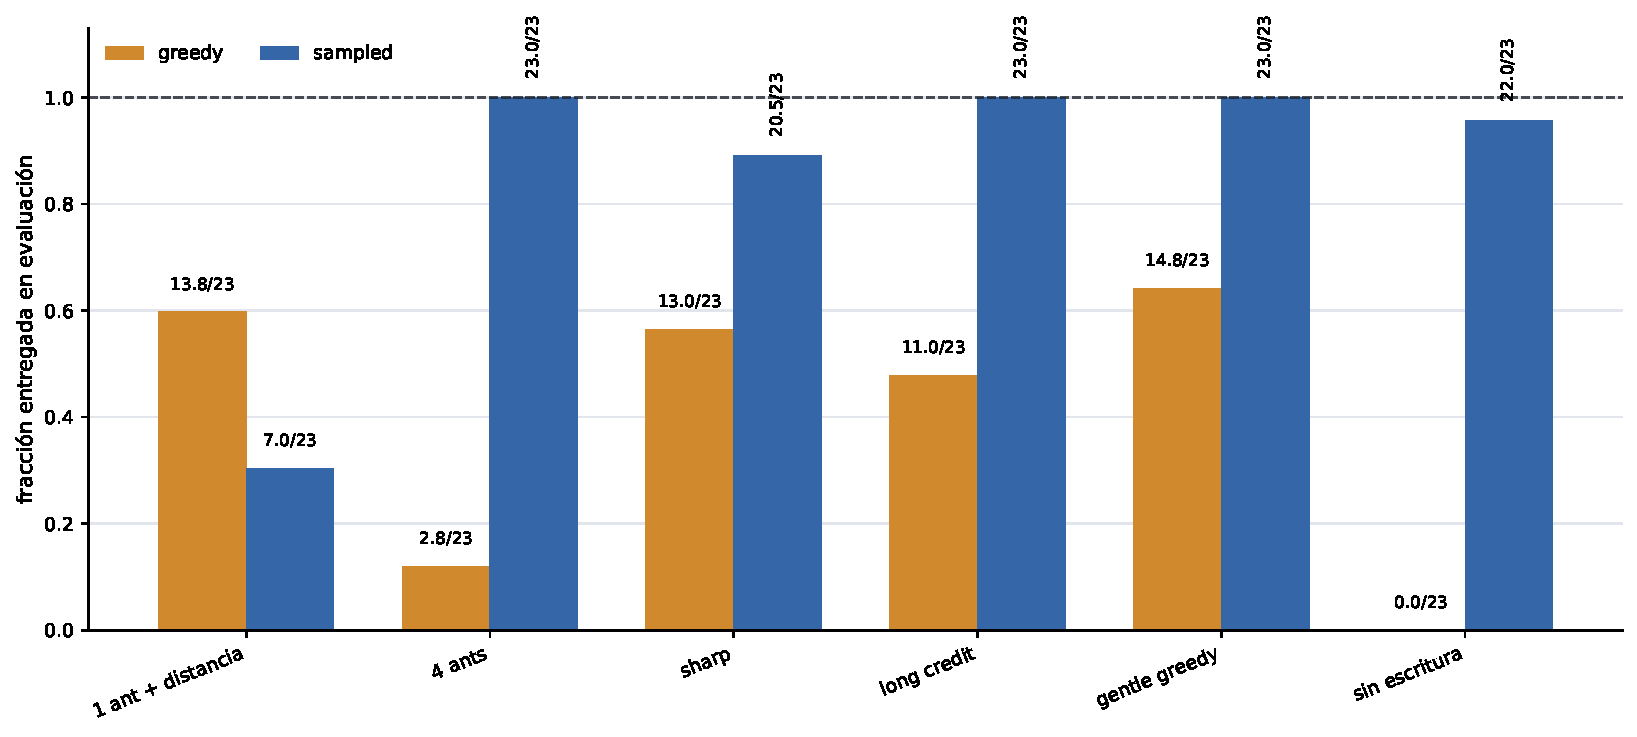
\includegraphics[width=\linewidth]{fig_25x25_modes.pdf}
\caption{Evaluación 25x25 bajo dos protocolos de despliegue. Cada barra muestra la fracción de comida entregada y anota entregas sobre 23 unidades. La línea punteada marca la tarea completa: el resultado importante es la brecha entre movimiento greedy y movimiento muestreado, no solo el máximo alcanzado.}
\label{fig:25x25}
\end{figure}

El resultado \run{DISTANCE_CAP4_NO_WRITE} es una advertencia contra sobreinterpretar comunicación: incluso sin escritura, una continuación entrega \(22/23\) bajo movimiento muestreado. No es una ablación perfectamente controlada, porque también cambian schedule y optimizador, pero sí muestra que la solución 25x25 no requiere demostrar comunicación por bytes.

Las continuaciones de 25x25 muestran que el problema no era un solo interruptor. \run{DISTANCE_CAP4_SHARP} mejora greedy a \(13/23\), pero baja el resultado muestreado a \(20.5/23\). La continuación long-credit recupera el \(23/23\) muestreado, aunque deja greedy en \(11/23\). La variante gentle-greedy sube greedy a \(14.75/23\) y conserva el \(23/23\) muestreado. \run{DISTANCE_VISION2_CAP4} también logra \(23/23\) muestreado con radio 2, pero cambia observación y capacidad. La lectura no es que una ablación aislada resolvió todo; es que shaping, cobertura, capacidad y modo de despliegue formaron un paquete aprendible.

\subsection{Bits contra cobertura}

Los barridos tempranos de bits no muestran un salto claro de capacidad. En una línea 15x15 aproximada, el retorno de entrenamiento sube de \(6.40\) a \(7.36\) al pasar de 2 a 5 bits y luego baja levemente en 8 bits. En la línea anclada a 25x25, el retorno se mantiene bajo. En cambio, aumentar el número de hormigas en 25x25 con 3 bits produce una mejora monotónica de retorno de episodio: \(7.7875\) con 2 hormigas, \(10.6987\) con 3, \(12.545\) con 4, \(16.1287\) con 6 y \(18.2294\) con 8.

\begin{figure}[h]
\centering
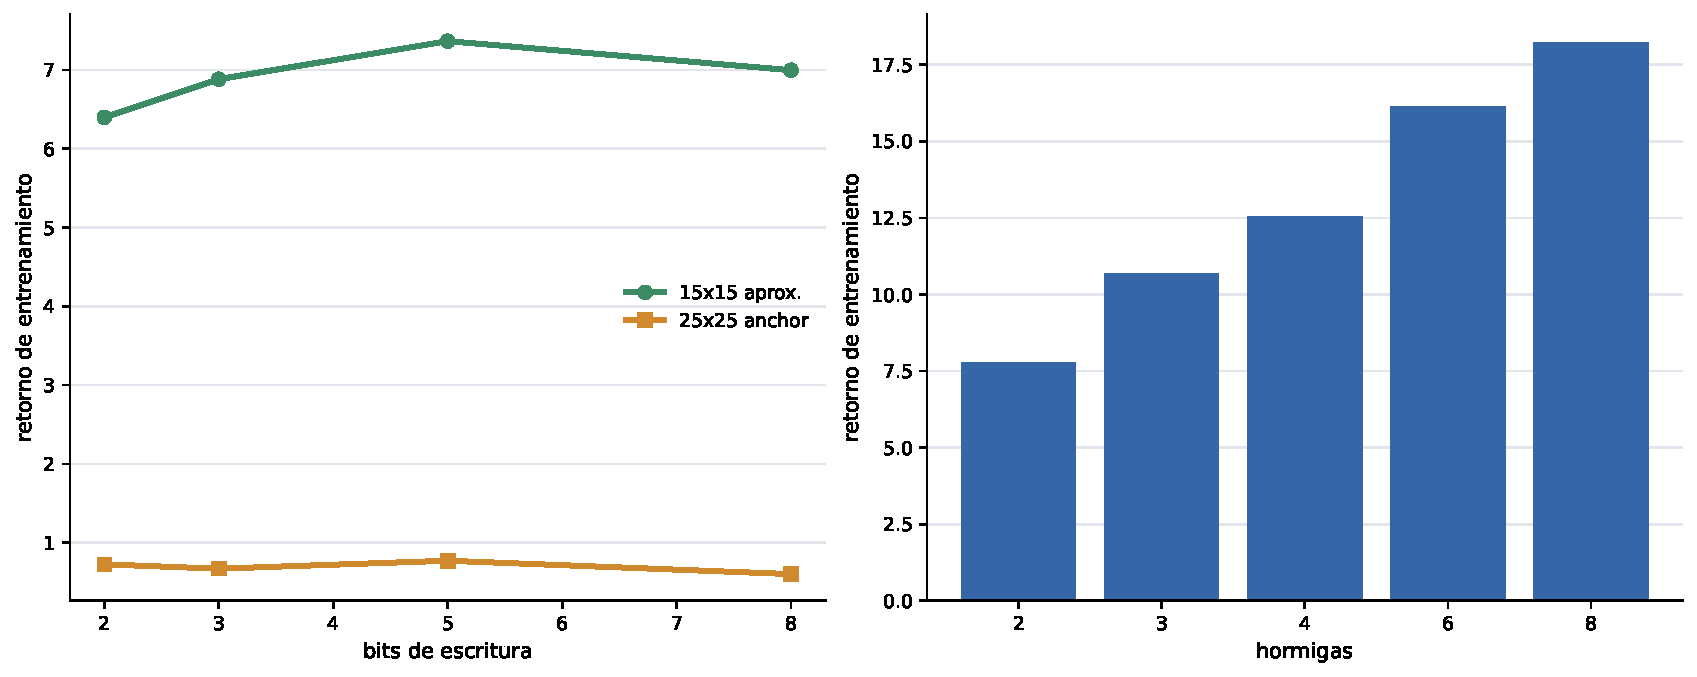
\includegraphics[width=\linewidth]{fig_bits_vs_ants.pdf}
\caption{Comparación entre dos hipótesis tempranas. El panel izquierdo muestra retornos de entrenamiento al variar la cantidad de bits de escritura; el panel derecho muestra retornos al variar la cantidad de hormigas. La lectura favorece una explicación de cobertura multi-agente antes que una explicación basada solo en aumentar el alfabeto de escritura. Estas curvas no son evaluaciones held-out.}
\label{fig:bits-ants}
\end{figure}

\subsection{Métricas registradas más allá del retorno final}

Las corridas locales y los resúmenes W\&B no registraban solo reward final. En varias ramas se guardaron \metric{delivery_events}, \metric{pickup_events}, \metric{mean_carrying_ants}, cobertura visitada, fracción de bytes no-cero, tasa de escritura, entropía, \metric{approx_kl}, norma de gradiente, \metric{value_loss} y, cuando había evaluación, comida entregada por 1000 pasos-hormiga. Esa instrumentación es parte de la historia: permitió detectar políticas que exploraban casi todo el mapa, escribían mucho o cargaban comida, pero no necesariamente entregaban.

En la línea 50x50 larga, por ejemplo, la cobertura final sube desde \(0.059\) al principio hasta \(0.9275\) hacia el final, mientras la tasa de escritura no-cero baja desde \(0.113\) hasta \(0.0168\). En la línea eficiente 50x50, los logs de evaluación registran eficiencia: una evaluación temprana dio \(13.5\) entregas y \(0.54\) entregas por 1000 pasos-hormiga; otra alcanzó \(18.0\) y \(0.72\), aunque más tarde esa familia volvió a oscilar. Estos números explican por qué el informe no debe contar solo el mejor video.

\begin{figure}[h]
\centering
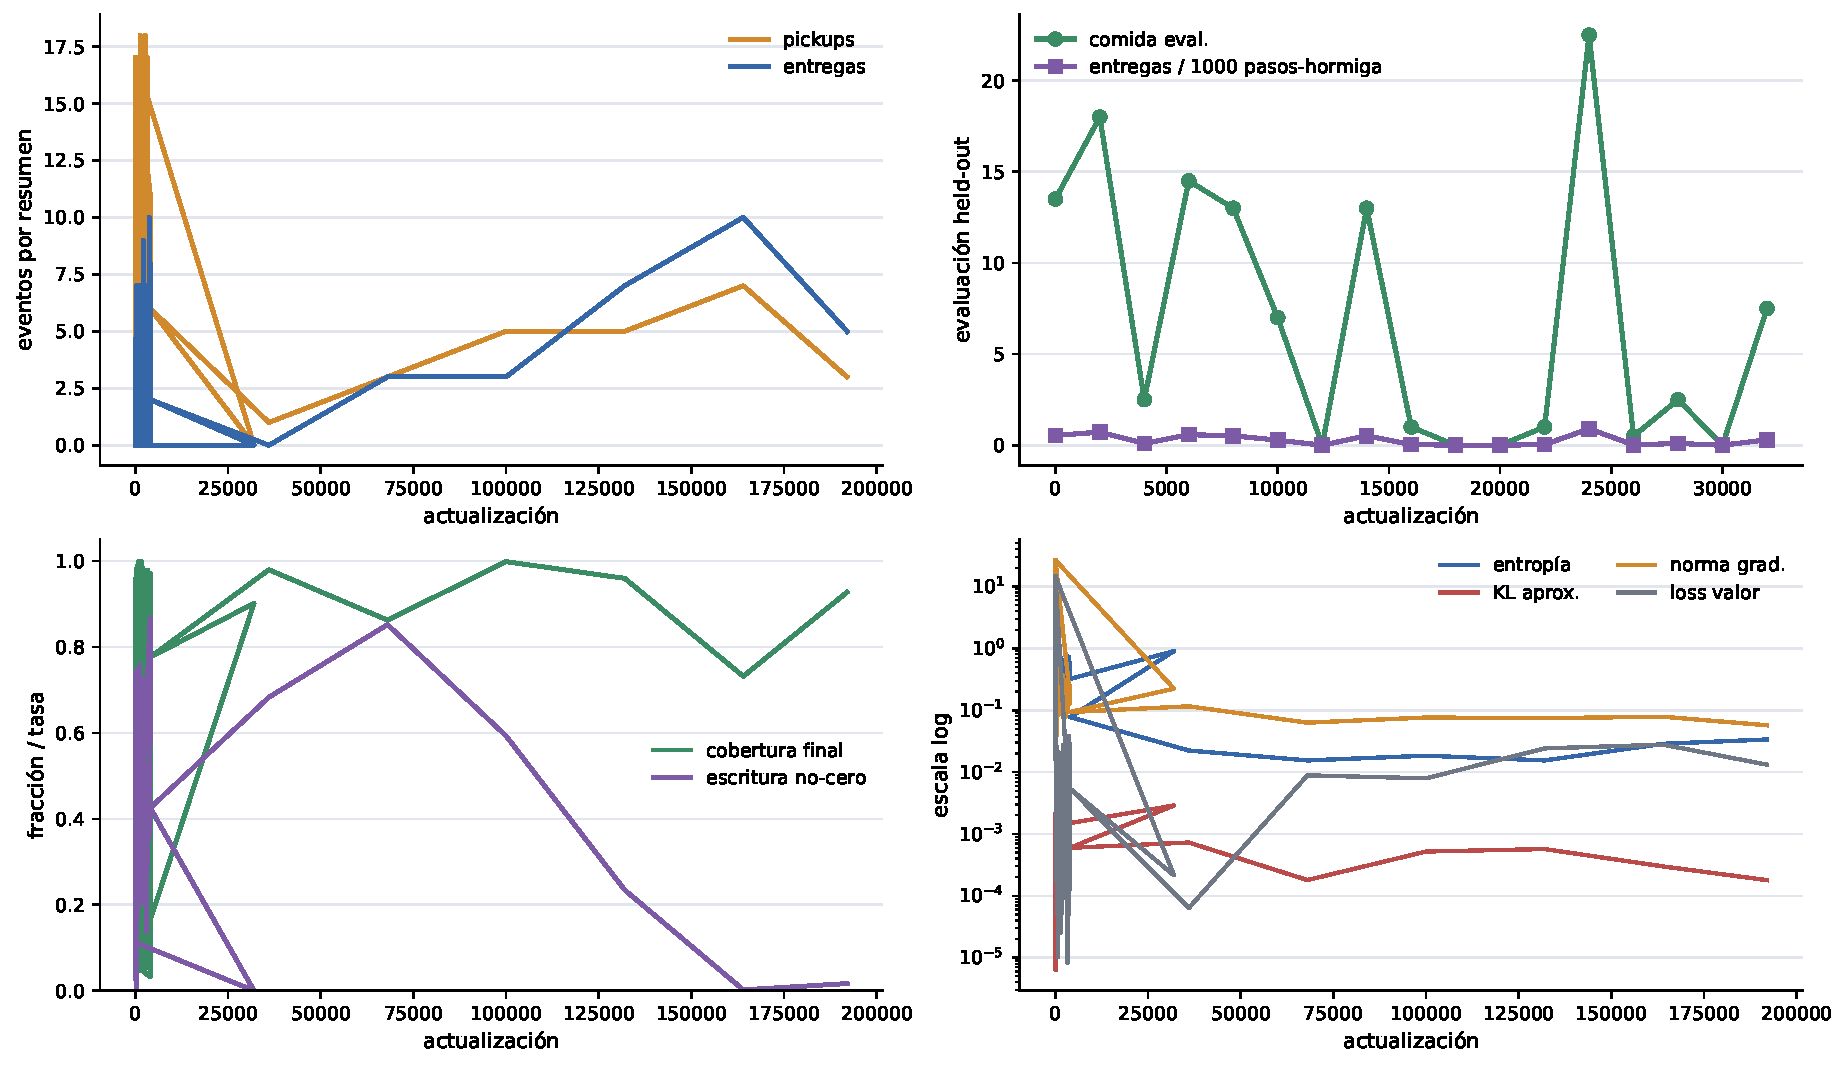
\includegraphics[width=\linewidth]{fig_logged_metrics_story.pdf}
\caption{Métricas registradas en logs locales de dos ramas 50x50. Los paneles separan eventos de tarea, evaluación held-out, cobertura/escritura y señales de optimización. La figura no reemplaza las tablas finales: muestra por qué el análisis necesita más dimensiones que retorno final o apariencia visual.}
\label{fig:logged-metrics}
\end{figure}

\subsection{Autocurriculum por tamaño activo}

La inspiración era el autocurriculum de locomoción de Rudin et al. en ETH Zurich \cite{rudin2022learning}. Allí el robot ANYmal no empieza resolviendo directamente los terrenos más difíciles. Miles de robots simulados se distribuyen por tipo de terreno y nivel de dificultad: plano, pendientes, rugosidad, obstáculos y escaleras. Si un robot cruza su terreno, en el siguiente reset sube de nivel; si no avanza lo suficiente, baja. En escaleras y obstáculos aumenta la altura del escalón, y en pendientes aumenta la inclinación. La idea útil para este proyecto era esa regla de control de dificultad: mantener al agente cerca de una frontera aprendible y endurecer el entorno solo cuando el comportamiento actual ya domina la etapa.

Nuestro autocurriculum por tamaño activo aplicó esa idea a una grilla 50x50 acolchada. La observación conservaba el formato final, pero el área jugable empezaba en 4x4 y crecía de a una celda por lado después de seis entregas en la etapa. El contrato relevante era una política de una hormiga, 12 unidades de comida, 2 fuentes, 1 bit de escritura, radio de visión 1, crítico \run{mlp}, \metric{pickup_bonus}=0.25 y sin moldeado de distancia. El objetivo era evitar entrenar una política distinta por tamaño: primero cerrar el ciclo fuente--hub en pequeño, después exigir el mismo ciclo en regiones cada vez más grandes hasta 50x50.

La reproducción de verificación en Google Cloud, resumida en \run{autocurriculum_active_size_gcloud.csv} y sincronizada a W\&B como \run{e5ymgvil}, confirma que la idea avanzaba etapas pero no cerraba el problema. El run completó \(1.28\) millones de pasos con \run{metrics.jsonl}, \run{summary.json} y checkpoint final. La mejor ventana observada llegó a 6 etapas completadas y tamaño activo máximo 19; el resumen final quedó en \metric{autocurriculum_max_active_size}=19, \metric{autocurriculum_completed_stages}=3, \metric{delivery_events}=5, \metric{pickup_events}=6 y \metric{episode_return}=0.40625. Es decir, el umbral por entregas sí podía empujar el curriculum fuera del 4x4 inicial, pero la política no transfería el ciclo de foraging hasta 50x50 bajo una sola hormiga, radio local 1 y crítico plano. La rama queda como evidencia negativa temprana: el aumento automático de dificultad no reemplazó al moldeado de distancia, la cobertura por más agentes ni el cambio posterior a críticos espaciales.

\subsection{Laberintos: entrenamiento exploratorio sin foraging comparable}

Otra rama exploró laberintos. En la rama actual queda el config \run{maze_exploration_curriculum.json}: laberintos generados de 10x10 a 50x50, una hormiga, 48 unidades de comida, 12 fuentes, 2 bits, radio 1, crítico MLP, \metric{max_steps}=6250, 16 entornos por 80 pasos, \metric{reward_mode}=\run{explore}, pasillos de ancho 3, paredes de ancho 1 y semilla 17. La infraestructura de obstáculos sí quedó implementada y testeada: obstáculos bloquean movimiento, aparecen en observaciones, los resets ubican hub/comida/hormigas en celdas abiertas y los layouts pueden cambiar tras truncación.

\begin{figure}[h]
\centering
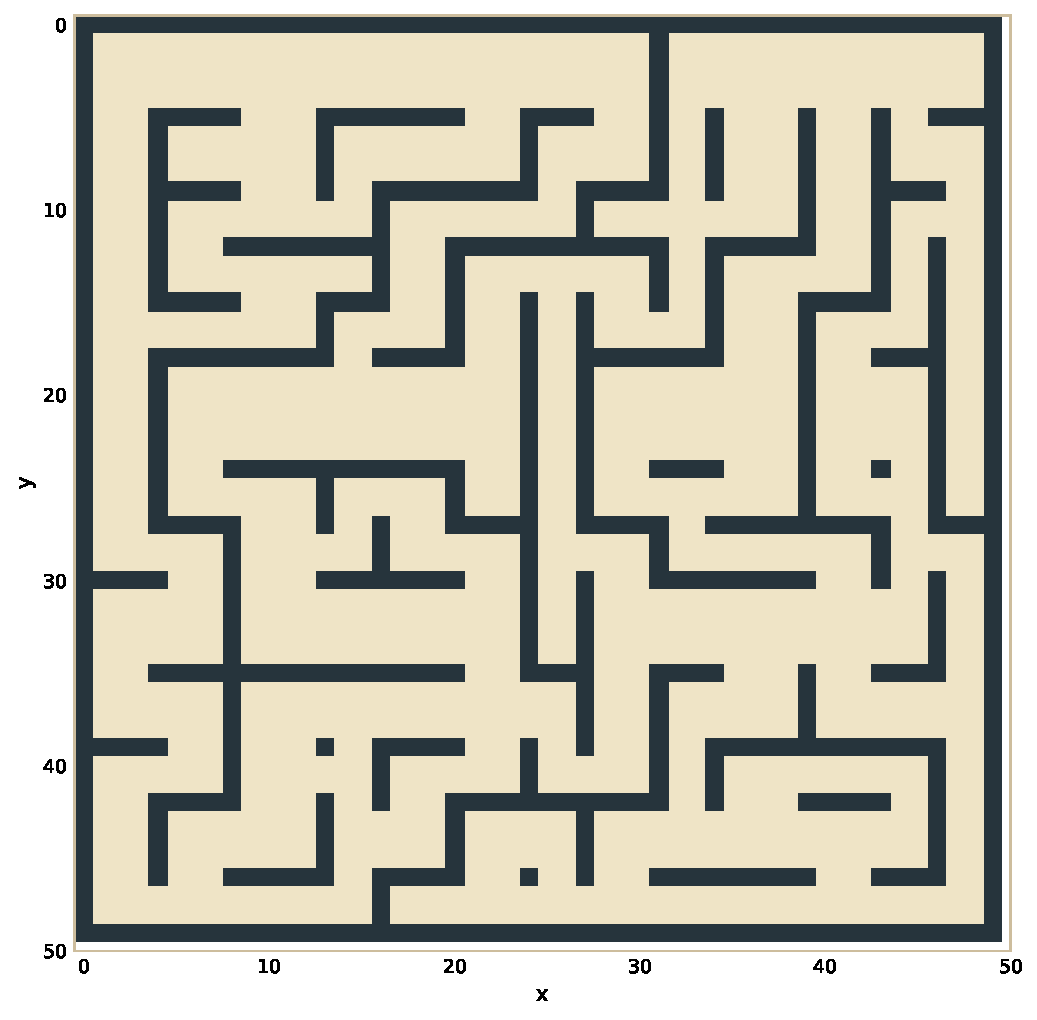
\includegraphics[width=0.82\linewidth]{fig_maze_layout.pdf}
\caption{Layout 50x50 generado desde \run{maze_exploration_curriculum.json} con el generador real de laberintos del entorno. Esta figura muestra la geometría; el sitio web complementa con el video W\&B 50x50 del currículo entrenado.}
\label{fig:maze-layout}
\end{figure}

También existió una rama lateral \run{origin/lethal_cookies}. Allí el cuaderno de maze preparaba una prueba de estrés 41x41 en forma de L dentro de una arena 50x50, con pasillos de ancho 5, 20 hormigas, una fuente normal al final y, en una variante hermana, bolsillos laterales para fuentes letales. Sin embargo, esa rama no tiene en el checkout actual métricas locales preservadas de entrega, supervivencia, eficiencia o convergencia, y la llamada de entrenamiento del cuaderno de maze estaba comentada.

Para el sitio web se recuperó el video correcto desde W\&B, correspondiente al run terminado \run{8ebnjq9f} y a la clave \run{videos/maze_exploration/50x50}. Ese artefacto sí viene de la política entrenada para laberintos: 50x50, una hormiga, 48 unidades de comida, 12 fuentes, 2 bits, radio 1, \metric{reward_mode}=\run{explore}, pasillos de ancho 3, paredes de ancho 1 y semilla 17. El MP4 tiene 600 fotogramas, \(800\times800\) píxeles, 8 fps y 75 segundos. El summary final reporta \metric{episode_return}=26.125, \metric{final_mean_remaining_food}=45.5/48 y \metric{completed_episodes}=0. La colección de modelos recuperable conserva checkpoints de laberinto hasta \run{jax_mappo_maze_explore_24x24.pkl}; para la etapa 50x50 quedó preservado el video, no el checkpoint local.

Después del cierre inicial del sitio se agregó una prueba de estrés no entrenada para laberinto: el actor estabilizado 50x50 de 60 hormigas se desplegó como solo-actor en un laberinto 100x100 con una sola fuente lejana. Se usó \run{sampled_move_greedy_write}, temperatura de movimiento \(0.525\) y escritura greedy. El hub quedó en \([6,5]\), la fuente efectiva en \([81,70]\), y en el layout seleccionado la distancia por pasillos fue 172. Las paredes sí entraron al actor por el mismo canal local de borde/obstáculo. Aun así, en 60000 pasos no hubo recogidas ni entregas: \(0/125\) entregado, \(125/125\) restante, 887 celdas visitadas y 886 celdas con bytes no-cero. Esta prueba no contradice el video entrenado de W\&B; muestra que el actor abierto de 60 hormigas no transfiere directamente a paredes internas aunque pueda observarlas.

Por eso el laberinto debe contarse como rama entrenada de exploración, no como resultado comparable de foraging cooperativo. La prueba 100x100 debe contarse como fallo de transferencia solo-actor, no como fallo de percepción de paredes. La infraestructura de obstáculos funcionó y produjo evidencia visual, pero el contrato entrenado de laberinto no medía entrega; la decisión experimental fue volver al foraging abierto, donde sí existían curvas, videos, puntos guardados y métricas de comida recolectada.

\subsection{Memoria y autoresearch: escribir no basta}

La línea de memoria intentó convertir la observación cualitativa de bytes escritos en una afirmación causal. El criterio correcto era más exigente: una política con bytes debía superar pruebas \run{no_byte_read} y \run{no_write}, y al mismo tiempo mantener o mejorar comida entregada. Los barridos R8--R12 y las recompensas \run{delivery_byte_trail_bonus}, \run{byte_follow_bonus} y variantes relacionadas fueron diseñados para esa pregunta.

\begin{figure}[h]
\centering
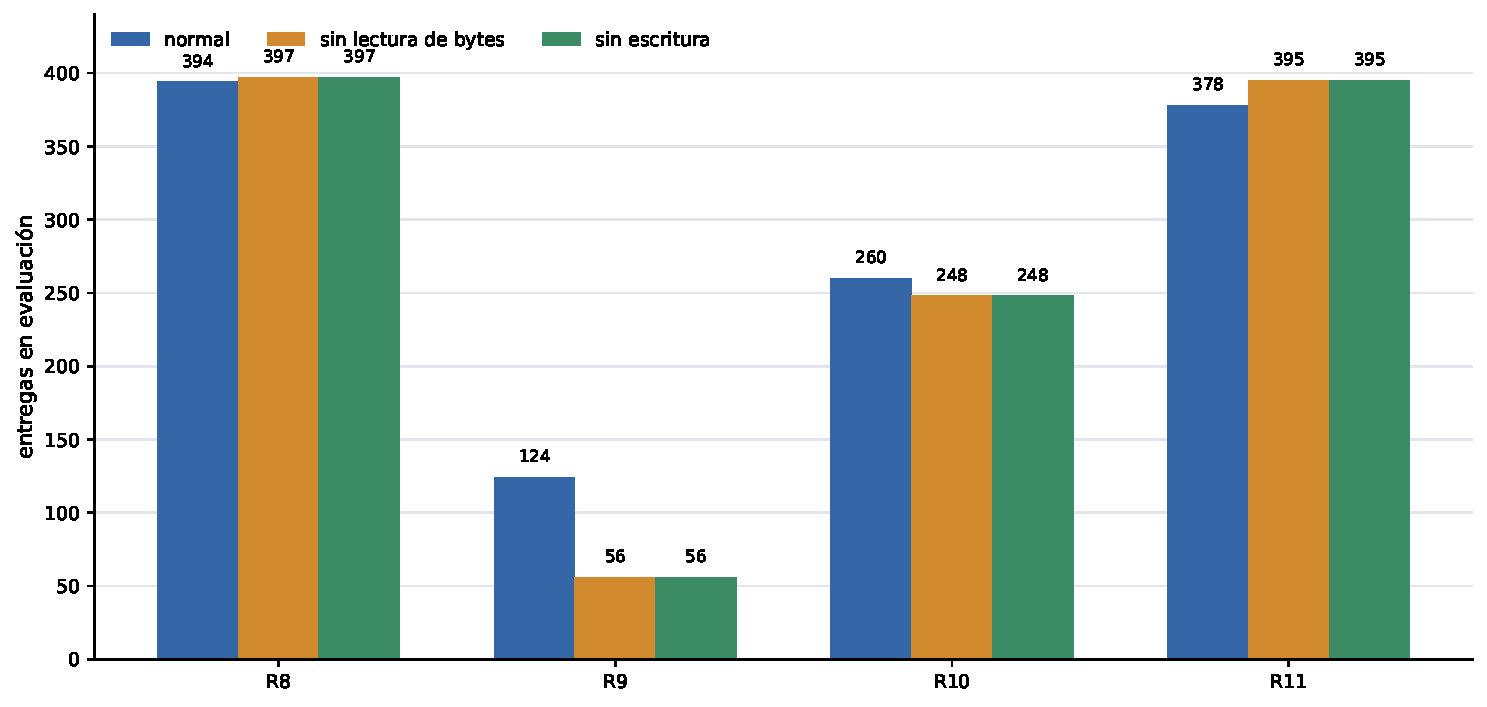
\includegraphics[width=\linewidth]{fig_memory_r8_r12_ablation.pdf}
\caption{Pruebas de memoria R8--R11. Cada grupo compara la evaluación normal contra dos ablaciones: impedir la lectura de bytes y bloquear la escritura. R12 queda fuera de la figura porque se interrumpió antes de un resultado final confiable. La lectura importante no es cuántos bytes aparecen, sino si la política mantiene foraging y mejora frente a las ablaciones.}
\label{fig:memory-r8-r12}
\end{figure}

La conclusión no fue positiva. El punto guardado sparse apenas dependía de los bytes. R8 entregó bien pero no a través de memoria: \run{normal}=394, \run{no_byte_read}=397 y \run{no_write}=397. R9 produjo una brecha más causal, pero dañó el foraging: \run{normal}=124 contra ablaciones de 56. R10 fue más liviano, aunque todavía débil: 260 contra 248. R11 preservó conducta sparse sin ganancia causal: 378 contra 395 y 395. R12 quedó interrumpido antes de un resultado final confiable. Junto con el resultado \run{DISTANCE_CAP4_NO_WRITE} de \(22/23\), esto impide afirmar que la memoria externa causó los mejores resultados. Lo que sí queda demostrado es más modesto: el entorno ofrece una memoria discreta y las políticas pueden escribirla; falta probar que esa información escrita mejore decisiones de forma robusta.

\subsection{Fuentes cada vez más dispersas}

Otra línea importante no escalaba por tamaño de mapa, sino por geometría de comida. La hipótesis era que el cuello de botella podía ser descubrimiento de fuentes: si la comida empieza fácil de encontrar y luego se vuelve escasa, quizá la política aprenda búsqueda y explotación sin depender tanto de ayudas de distancia.

Hubo varias formas de probarlo. \run{exploration_to_forage_padded_sources_50x50} mantuvo una arena 50x50 por compatibilidad de checkpoint, restringió hub y comida a una ventana interior 20x20, partió de un checkpoint 20x20 y redujo posiciones de fuente de 12 a 2 con 18 unidades totales. Esa forma fue débil: alrededor de \(0.25/18\). \run{exploration_to_forage_scratch_smooth_sources_50x50} fue más ambiciosa: arena exterior 80x80, ventana interior 50x50, 250 unidades de comida, 4 bits y annealing suave de posiciones de fuente desde 250 hasta 2. No quedó como resultado principal. \run{exploration_to_forage_proximity_sources_50x50} cambió la idea: mantener dos macro-fuentes desde el inicio, pero empezar con footprints cercanos y reducirlos hasta dos celdas finales dentro de una ventana interior 30x30.

El resultado de proximidad llegó a \(40.875/250\), pero no debe leerse aislado: esa rama también introduce el crítico espacial \run{strided_cnn}. Por eso el currículo de fuentes dispersas es una pieza de la historia, no una conclusión causal cerrada. Mostró que descubrimiento de comida y representación espacial del crítico eran cuellos distintos.

\begin{table}[h]
\centering
\caption{Currículos de tamaño y de fuentes dispersas.}
\begin{tabularx}{\linewidth}{>{\raggedright\arraybackslash}p{0.24\linewidth}X>{\raggedright\arraybackslash}p{0.24\linewidth}}
\toprule
Rama & Contrato & Lectura \\
\midrule
\run{forage_curriculum} & 1 hormiga, 4x4--50x50, 48 comidas, 12 fuentes, 1 bit. & Primer enfoque por mapas crecientes; colapsa al crecer. \\
\run{autocurriculum} & cuadrado activo 4x4--50x50, avance tras 6 entregas por etapa, 12 comidas en 2 fuentes. & Avanza etapas, pero no produce competencia transferible robusta. \\
\run{padded_sources} & 50x50 oculto, ventana interior 20x20, posiciones de fuente 12--2, 18 comidas. & Resultado débil, cerca de \(0.25/18\). \\
\run{smooth_sources} & 80x80 exterior, 50x50 interior, 250 comidas, posiciones 250--2. & Prueba de annealing suave; no queda como resultado principal. \\
\run{proximity_sources} & 50x50 exterior, 30x30 interior, 4 hormigas, 250 comidas, dos macro-fuentes con footprint decreciente. & \(40.875/250\), mezclado con \run{strided_cnn}. \\
\bottomrule
\end{tabularx}
\end{table}

\subsection{Ablaciones y diagnósticos que cambiaron la interpretación}

No todas las ramas fueron resultados principales, pero varias cambiaron qué se podía afirmar. La regla de lectura fue conservadora: cuando una corrida cambia muchas cosas a la vez, se cuenta como intervención; cuando compara una política contra una versión \run{no_write}, \run{no_byte_read} o un costo equivalente, se acerca más a una ablación causal.

\begin{table}[h]
\centering
\footnotesize
\caption{Diagnósticos que evitaron sobreinterpretar el resultado principal.}
\begin{tabularx}{\linewidth}{>{\raggedright\arraybackslash}p{0.20\linewidth}>{\raggedright\arraybackslash}p{0.23\linewidth}>{\raggedright\arraybackslash}p{0.20\linewidth}X}
\toprule
Diagnóstico & Cambio & Número clave & Lectura \\
\midrule
\run{DISTANCE_CAP4_NO_WRITE} & 25x25 sin escritura. & muestreado \(22/23\), éxito \(0.5\). & La política 25x25 no necesita demostrar comunicación por bytes para explicar el solve muestreado. \\
R8--R12 memoria & \run{normal} contra \run{no_byte_read} y \run{no_write}. & R8 \(394/397/397\); R9 \(124/56/56\). & La dependencia causal aparece cuando el foraging empeora; no prueba una memoria útil y robusta. \\
Escritura compartida y costo & 8 hormigas 50x50 con escritura compartida y penalización. & \(45.25/125\) a \(69.375/125\). & Progreso práctico en el linaje \run{strided_cnn}, no ablación aislada. \\
Sondeo de comunicación & Evaluación del checkpoint con costo de escritura. & determinista \(18.5/125\), muestreado \(22.25/125\). & Los bytes existen, pero la lectura causal sigue débil. \\
Costo de escritura x300 / 6 fuentes & Costo severo y fuentes más numerosas. & primer eval \(68.375/125\), final \(19.625/125\). & Reducir escritura puede degradar la política si el contrato cambia demasiado. \\
250x250 trunc4096 & Continuación desde frontera con horizonte truncado. & mejor train \(685\), final \(13\). & Hubo picos, pero no estabilidad final. \\
Directa / exploración / laberinto & Líneas base e infraestructura lateral. & video W\&B 50x50; prueba 100x100: 0 recogidas, 0 entregas. & La rama entrenada era exploración; la prueba solo-actor muestra no-transferencia al laberinto. \\
\bottomrule
\end{tabularx}
\end{table}

\subsection{50x50 raro y ayudas vectoriales}

Cuando la comida se vuelve rara en 50x50, el problema cambia. El agente debe descubrir fuentes con baja probabilidad y luego sostener ciclos. La línea base rara llega a \(10.96/23\). Agregar visión de radio 2 no ayuda. Agregar vector al hub mejora poco. Agregar vector al hub y a la comida cercana sube a \(15.20/23\), y selección held-out llega a \(16.20/23\) en la confirmación final. La rama posterior de radio de spawn fue inconclusa, no negativa: completó \run{spawn8} con retorno de entrenamiento 5.898, \run{spawn16} con 7.209 y se detuvo en \(130/500\) actualizaciones de la etapa final sin \run{summary.json}.

\begin{figure}[h]
\centering
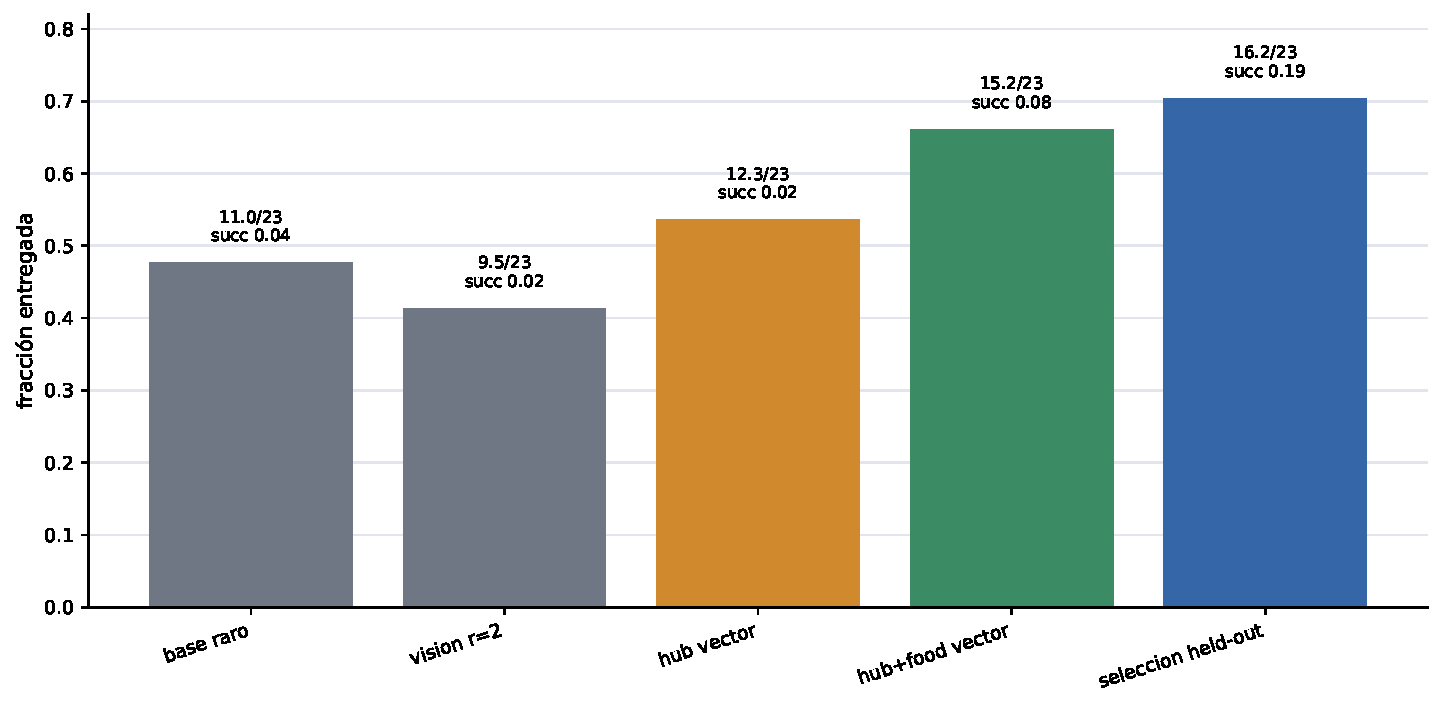
\includegraphics[width=0.9\linewidth]{fig_rare_50x50.pdf}
\caption{Evaluaciones seleccionadas en el escenario 50x50 con fuentes raras. Las barras reportan fracción entregada y anotan entregas sobre 23 junto con tasa de éxito. Las ayudas vectoriales parecen facilitar descubrimiento, pero la mejora no prueba comunicación emergente porque las corridas cambian más de una variable.}
\label{fig:rare}
\end{figure}

\subsection{La frontera del crítico en 50x50}

La línea 50x50 eficiente inicial usa el crítico MLP por defecto y entrega \(21.5/48\). La línea posterior de proximidad y full-layout cambia a \run{strided_cnn}. Ese cambio es mayor: el crítico ya no procesa una observación central plana, sino una representación espacial. Dentro de esa familia aparecen mejoras importantes, pero también colapsos de checkpoint y fuerte dependencia de selección.

\begin{figure}[h]
\centering
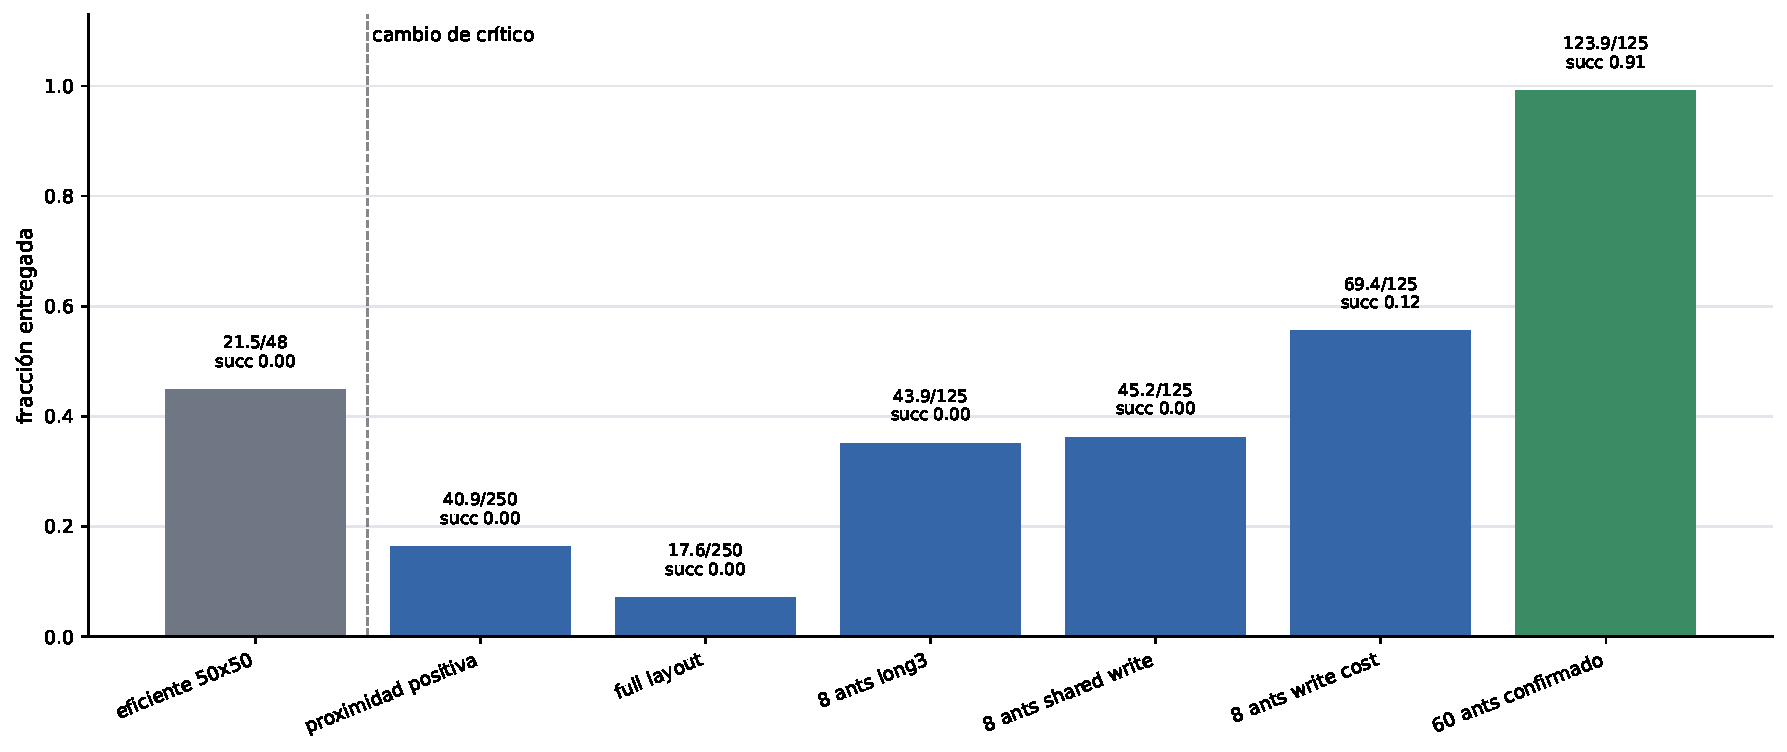
\includegraphics[width=\linewidth]{fig_critic_50x50.pdf}
\caption{Resultados 50x50 seleccionados con denominadores explícitos en cada barra. La línea vertical marca el cambio de crítico MLP a crítico espacial. Las barras posteriores no son una sola ablación: combinan arquitectura del crítico, geometría de fuentes, cantidad de hormigas, escritura, costos y selección de checkpoints.}
\label{fig:critic50}
\end{figure}

El mejor resultado local de 8 hormigas en esa familia es \run{shared_writes_write_cost_from_shared_best}: \(69.375/125\), éxito \(0.125\). Es progreso real, pero no una solución completa. También tiene escritura no-cero muy alta, alrededor de \(0.94\), por lo que no alcanza para afirmar que haya un código compacto e interpretable.

La línea reciente de 60 hormigas es la frontera actual del repo. Una evaluación de 64 episodios del punto guardado estabilizado reporta \(123.90625/125\), fracción \(0.99125\), éxito \(0.90625\). Esto es fuerte como ingeniería de comportamiento 50x50, pero cambia demasiadas cosas a la vez: 60 hormigas, 8 bits, actor con identidades repetidas, continuación desde un punto guardado, crítico \run{strided_cnn}, selección por evaluación, temperaturas y escritura casi saturada. Debe presentarse como resultado prometedor, no como prueba causal de comunicación.

\subsection{250x250: la trampa del retorno moldeado}

La escala 250x250 mostró el fracaso más informativo. Corridas con \run{resnet_cnn} o \run{strided_cnn} en una fuente terminan con cero pickups y cero entregas. En la familia \run{set_cnn}, el autocurrículo de distancia puede producir retorno positivo de moldeado, muchos agentes cargando y mapas de bytes saturados, pero todavía cero entregas finales. Es exactamente el tipo de resultado que un informe debe separar de la métrica objetivo.

\begin{figure}[h]
\centering
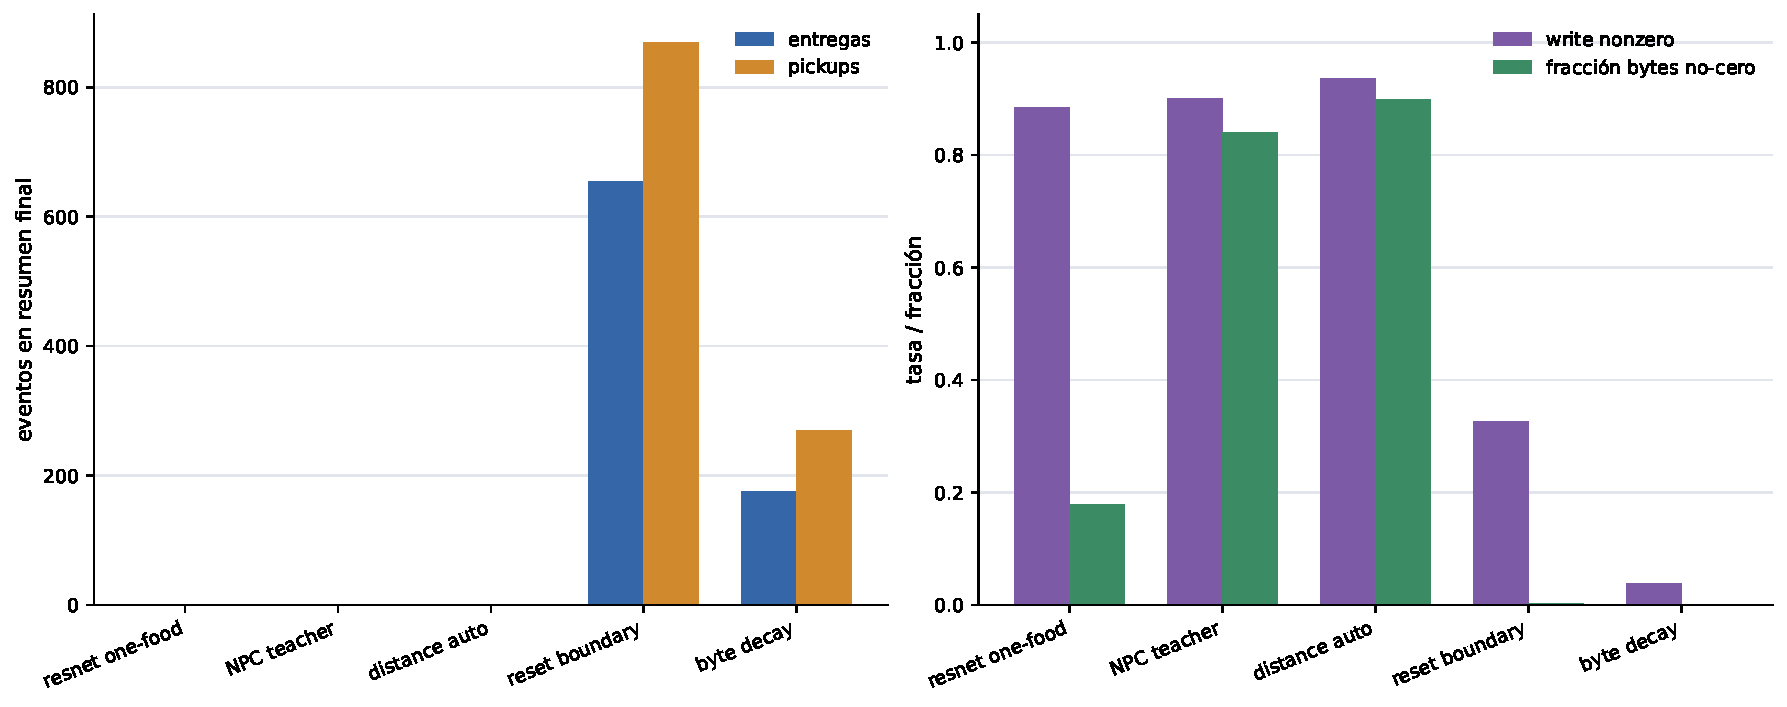
\includegraphics[width=\linewidth]{fig_250x250_diagnostics.pdf}
\caption{Diagnóstico 250x250 separado por métrica. El panel izquierdo muestra eventos reales de tarea, entregas y pickups. El panel derecho muestra actividad de escritura y fracción de bytes no-cero. La comparación deja visible la lección negativa: el retorno moldeado y la actividad de bytes pueden crecer sin resolver entrega; reset-boundary recupera progreso local de entrega.}
\label{fig:250}
\end{figure}

El cambio \run{fixed8-reset-boundary256} sí mejora la entrega local: el resumen final tiene \(654\) entregas y \(869\) pickups, y el mejor tramo de entrenamiento llega a alrededor de 1003 entregas. La evaluación fresh-window del mismo linaje selecciona \run{reset_boundary_final} como campeón por mediana de entregas. Aun así, esto no resuelve la escala general. Es una intervención de reset y distancia dentro de una familia de crítico distinta.

Las continuaciones posteriores refuerzan esa lectura. \run{byte-decay} redujo ocupación de bytes pero terminó con 175 entregas. La evaluación larga d12 de la rama no-decay mostró una media de 0.392 entregas, mediana 0, \metric{pickup_to_delivery_rate}=0.008 y 13.745 pickups no entregados en promedio. El intento estratificado d4/d8/d12 dejó manifiesto y configuración, pero los archivos \run{metrics.jsonl}, \run{fresh_eval_metrics.jsonl} y \run{long_eval_metrics.jsonl} quedaron vacíos después de un aborto operacional tipo exit 137. No es evidencia contra la hipótesis; simplemente no produjo un resultado interpretable.

\section{Evidencia cualitativa}

Los videos apoyan una lectura progresiva. Primero hay movimiento local sin retorno estable. Después, los rollouts preservados del currículo 25x25 muestran cómo cambia el comportamiento al pasar por 2, 3, 4, 6 y 8 hormigas: la cobertura deja de ser un detalle y se vuelve parte del mecanismo. En 50x50 con crítico espacial aparecen rutas repetidas y entregas más densas. Las visualizaciones grandes deben leerse con cuidado: 100x100 es una continuación seleccionada, 250x250 muestra una recuperación local por reset-boundary, y 1000x1000 es un despliegue solo-actor de una política ya entrenada, no entrenamiento de punta a punta en ese entorno. La prueba 100x100 de laberinto agrega una evidencia negativa visualmente útil: hay exploración local y escritura de bytes, pero no aparece el ciclo recogida--retorno que define el foraging.

\begin{figure}[h]
\centering

\includegraphics[width=\linewidth,height=0.72\textheight,keepaspectratio]{fig_behavior_montage.jpg}
\caption{Fotogramas extraídos de videos locales. A: línea base aleatoria. B--F: progresión visual del currículo 25x25 con 2, 3, 4, 6 y 8 hormigas. G: frontera 50x50 con 60 hormigas. H: despliegue solo-actor 1000x1000 de la política 50x50. La figura no es evidencia cuantitativa; sirve para interpretar la semántica visual de las métricas.}
\label{fig:behavior}
\end{figure}

\section{Discusión}

La evidencia más fuerte apunta a cinco decisiones que sí cambiaron el problema de manera productiva. La primera fue redefinir la tarea alrededor de entregas reales y fuentes agotables; sin esa frontera, una política podía parecer activa sin cerrar ciclos de foraging. La segunda fue usar moldeado de distancia para atravesar el horizonte largo inicial, especialmente en 25x25. La tercera fue aumentar la cobertura mediante más hormigas, un cambio que tuvo más efecto práctico que aumentar simplemente la cantidad de bits. La cuarta fue evaluar políticas con movimiento muestreado cuando el comportamiento aprendido vivía en la distribución y no en el argmax. La quinta, crucial para 50x50, fue reemplazar el crítico centralizado plano por una arquitectura espacial.

Otros resultados son útiles, pero tienen confusión causal. La escritura compartida y las penalizaciones de escritura mejoraron algunas continuaciones 50x50, aunque no aislaron el rol de los bytes. El aumento a 8 bits tampoco es una ablación limpia, porque cambió junto con costos, cantidad de hormigas y selección de checkpoints. La línea de 60 hormigas es el resultado conductual más fuerte, pero mezcla 60 agentes, identidades repetidas, 8 bits, continuación desde un punto guardado, crítico \run{strided_cnn}, selección por evaluación y escritura casi saturada. En 250x250, \run{reset-boundary} arregla ventanas locales de entrenamiento, pero no demuestra que el autocurrículo general de gran escala haya quedado resuelto.

La evidencia negativa es igual de importante para la interpretación. Aumentar bits no funcionó como mecanismo único de escala. El autocurriculum por tamaño activo podía avanzar etapas sin llegar a 50x50, y en 250x250 el retorno moldeado podía crecer aunque las entregas reales siguieran siendo nulas. El flujo de laberintos produjo un video entrenado de exploración 50x50 y una prueba de estrés 100x100, pero no una demostración comparable de foraging cooperativo en laberinto. Las ramas R8--R12 mostraron que puede haber dependencia de bytes, pero no una mejora robusta de tarea causada por memoria externa. Las ramas adversariales, timed-release y lethal-cookies quedan ubicadas en el árbol por refs, commits e infraestructura, aunque no tienen el mismo paquete de métricas, videos y evaluaciones que las líneas centrales.

Por estas razones, el informe evita tres sobreinterpretaciones. El despliegue determinista no se usa como único criterio de éxito cuando la política aprendida es estocástica. El retorno moldeado no se trata como sustituto de entrega real. Y la comunicación emergente no se afirma sin ablaciones emparejadas, como \run{no_write}, bytes permutados, costos igualados entre alfabetos y comparaciones de crítico bajo el mismo contrato de entorno.

\section{Limitaciones}

La limitación principal es experimental: muchas corridas son continuaciones con varios cambios simultáneos. Por eso este informe habla de ``intervenciones'' y no de ablaciones puras salvo donde haya evidencia comparable. También hay diferencias entre punto guardado final, mejor punto guardado, selección held-out y resúmenes W\&B. Esas diferencias importan porque varias corridas tienen pico temprano y luego degradación.

La segunda limitación es semántica. La memoria externa existe y se usa en el sentido de que hay acciones de escritura y bytes no-cero. Pero todavía falta demostrar que la información escrita cause mejores decisiones. Para eso hacen falta evaluaciones como: congelar política y borrar bytes, permutar bytes entre celdas, bloquear escritura solo en test, igualar costos entre 4 y 8 bits, y comparar \run{mlp} contra \run{strided_cnn} con el mismo entorno.

La tercera limitación es de escala. El resultado 60-ant 50x50 es muy bueno, pero usa muchos agentes y escritura saturada. Puede ser la dirección de ingeniería correcta, pero no responde por sí solo la pregunta de comunicación compacta.

La cuarta limitación es de trazabilidad negativa. Algunas ramas importantes, como laberintos, lethal-cookies, roles adversariales, timed-release, multi-device/write-cost y cuadernos laterales de prueba de estrés, quedaron mejor representadas por código, commits, refs, videos diagnósticos y metadatos que por evaluaciones finales comparables. En este informe se incluyen porque explican decisiones del proyecto, pero no se usan como evidencia cuantitativa de desempeño. El video W\&B de laberinto y la prueba 100x100 muestran comportamiento, no una métrica de foraging cooperativo resuelta.

\section{Conclusión}

El proyecto produjo una historia clara. Primero hubo que corregir la semántica de la tarea: entregar comida, no solo encontrarla. Luego hubo que hacer aprendible el crédito: moldeado de distancia, más agentes y despliegue muestreado. Después apareció el detalle más importante para 50x50: el crítico centralizado espacial. Ese cambio reestructura el aprendizaje y debe figurar como una causa mayor. La memoria por bytes sigue siendo una hipótesis interesante, no una conclusión demostrada.

La contribución honesta del trabajo no es ``resolvimos comunicación emergente''. Es más precisa: construimos un entorno de foraging multi-agente con memoria externa, identificamos qué cambios desbloquean cada escala, alcanzamos solución robusta en 25x25 y resultados muy fuertes en 50x50 bajo crítico espacial, mostramos que en 250x250 el retorno moldeado puede engañar si no se mide entrega real, y dejamos un árbol auditado donde también figuran las ramas que fallaron, quedaron incompletas o solo sobreviven como infraestructura experimental.

\appendix
\section{Trabajo futuro}

El informe cierra la historia experimental disponible en el checkout actual, pero varias extensiones convertirían las lecturas principales en evidencia causal más fuerte. La primera prioridad es congelar una tabla canónica de runs y checkpoints por familia, acompañada por hiperparámetros comparables: \run{critic_architecture}, \run{food_count}, \run{food_sources}, cantidad de hormigas, bits, modo de evaluación y criterio de selección. Esa tabla evitaría que los resultados dependan de nombres de corrida o de memoria contextual.

La segunda prioridad es completar la trazabilidad externa. La auditoría actual garantiza exhaustividad local, pero la tabla cloud de W\&B debería regenerarse después de \run{wandb relogin}. También conviene inspeccionar manualmente el bucket \run{unclassified-review-needed} antes de usarlo como evidencia en un paper o presentación.

La tercera prioridad es ejecutar ablaciones emparejadas para memoria. Una prueba mínima debería comparar la misma política bajo escritura normal, escritura bloqueada, lectura bloqueada, bytes permutados entre celdas y costos igualados entre alfabetos de 4 y 8 bits. Si se quiere convertir los laberintos en una línea principal, el contrato también debe cambiar: no basta un video de exploración, sino que hace falta una plantilla comparable con recogidas, entregas, eficiencia, tiempo de convergencia, 60 hormigas y una fuente lejana bajo el mismo criterio de evaluación.

\bibliographystyle{plain}
\bibliography{references}

\end{document}
